
% This document is for the Group Meeting Agenda.  The Agenda should
% be distributed to each member (and other invitees) and to the TA
% prior to the meeting (hopefully the day before) so that each member
% will have adequate time to prepare for the meeting.  The best way
% to accomplish the distribution of the agenda is to email the LaTeX
% file to all members and TA.
%
%\documentstyle[fullpage]{article}
\documentclass[a4paper,12pt]{article}
\usepackage{fullpage}
\usepackage{cite}
\usepackage{url}
\usepackage{xcolor}
\usepackage{setspace}
\usepackage[version=4]{mhchem}
\usepackage{upgreek}
\usepackage[margin=0.75in]{geometry}
% For figure:
\usepackage{graphicx}
\usepackage{float}
% For table:
\usepackage{makecell}
\makeatletter
% we use \prefix@<level> only if it is defined
\renewcommand{\@seccntformat}[1]{%
  \ifcsname prefix@#1\endcsname
    \csname prefix@#1\endcsname
  \else
    \csname the#1\endcsname\quad
  \fi}
% define \prefix@section
\newcommand\prefix@section{}
\makeatother
\begin{document}

%
% This section gives the general information about the meeting such
% as the title, who it was called by, when and where the meeting
% will take place, what type of meeting it is (planning, design,
% problem-solving, decision-making, etc.), and of course who is
% invited to attend.
%

\pagestyle{fancyplain}
\fancyhf{}
\lhead{ \fancyplain{}{BIOL 4020 – Vertebrate Biodiversity - Diapsids}}
%\chead{ \fancyplain{}{}}
\rhead{ \fancyplain{}{Fall 2020}}
%\rfoot{\fancyplain{}{page \thepage\ of \pageref{LastPage}}}
\fancyfoot[RO, LE] {page \thepage\ of \pageref{LastPage}}
\thispagestyle{plain}

\begin{figure}[H]
\centering
  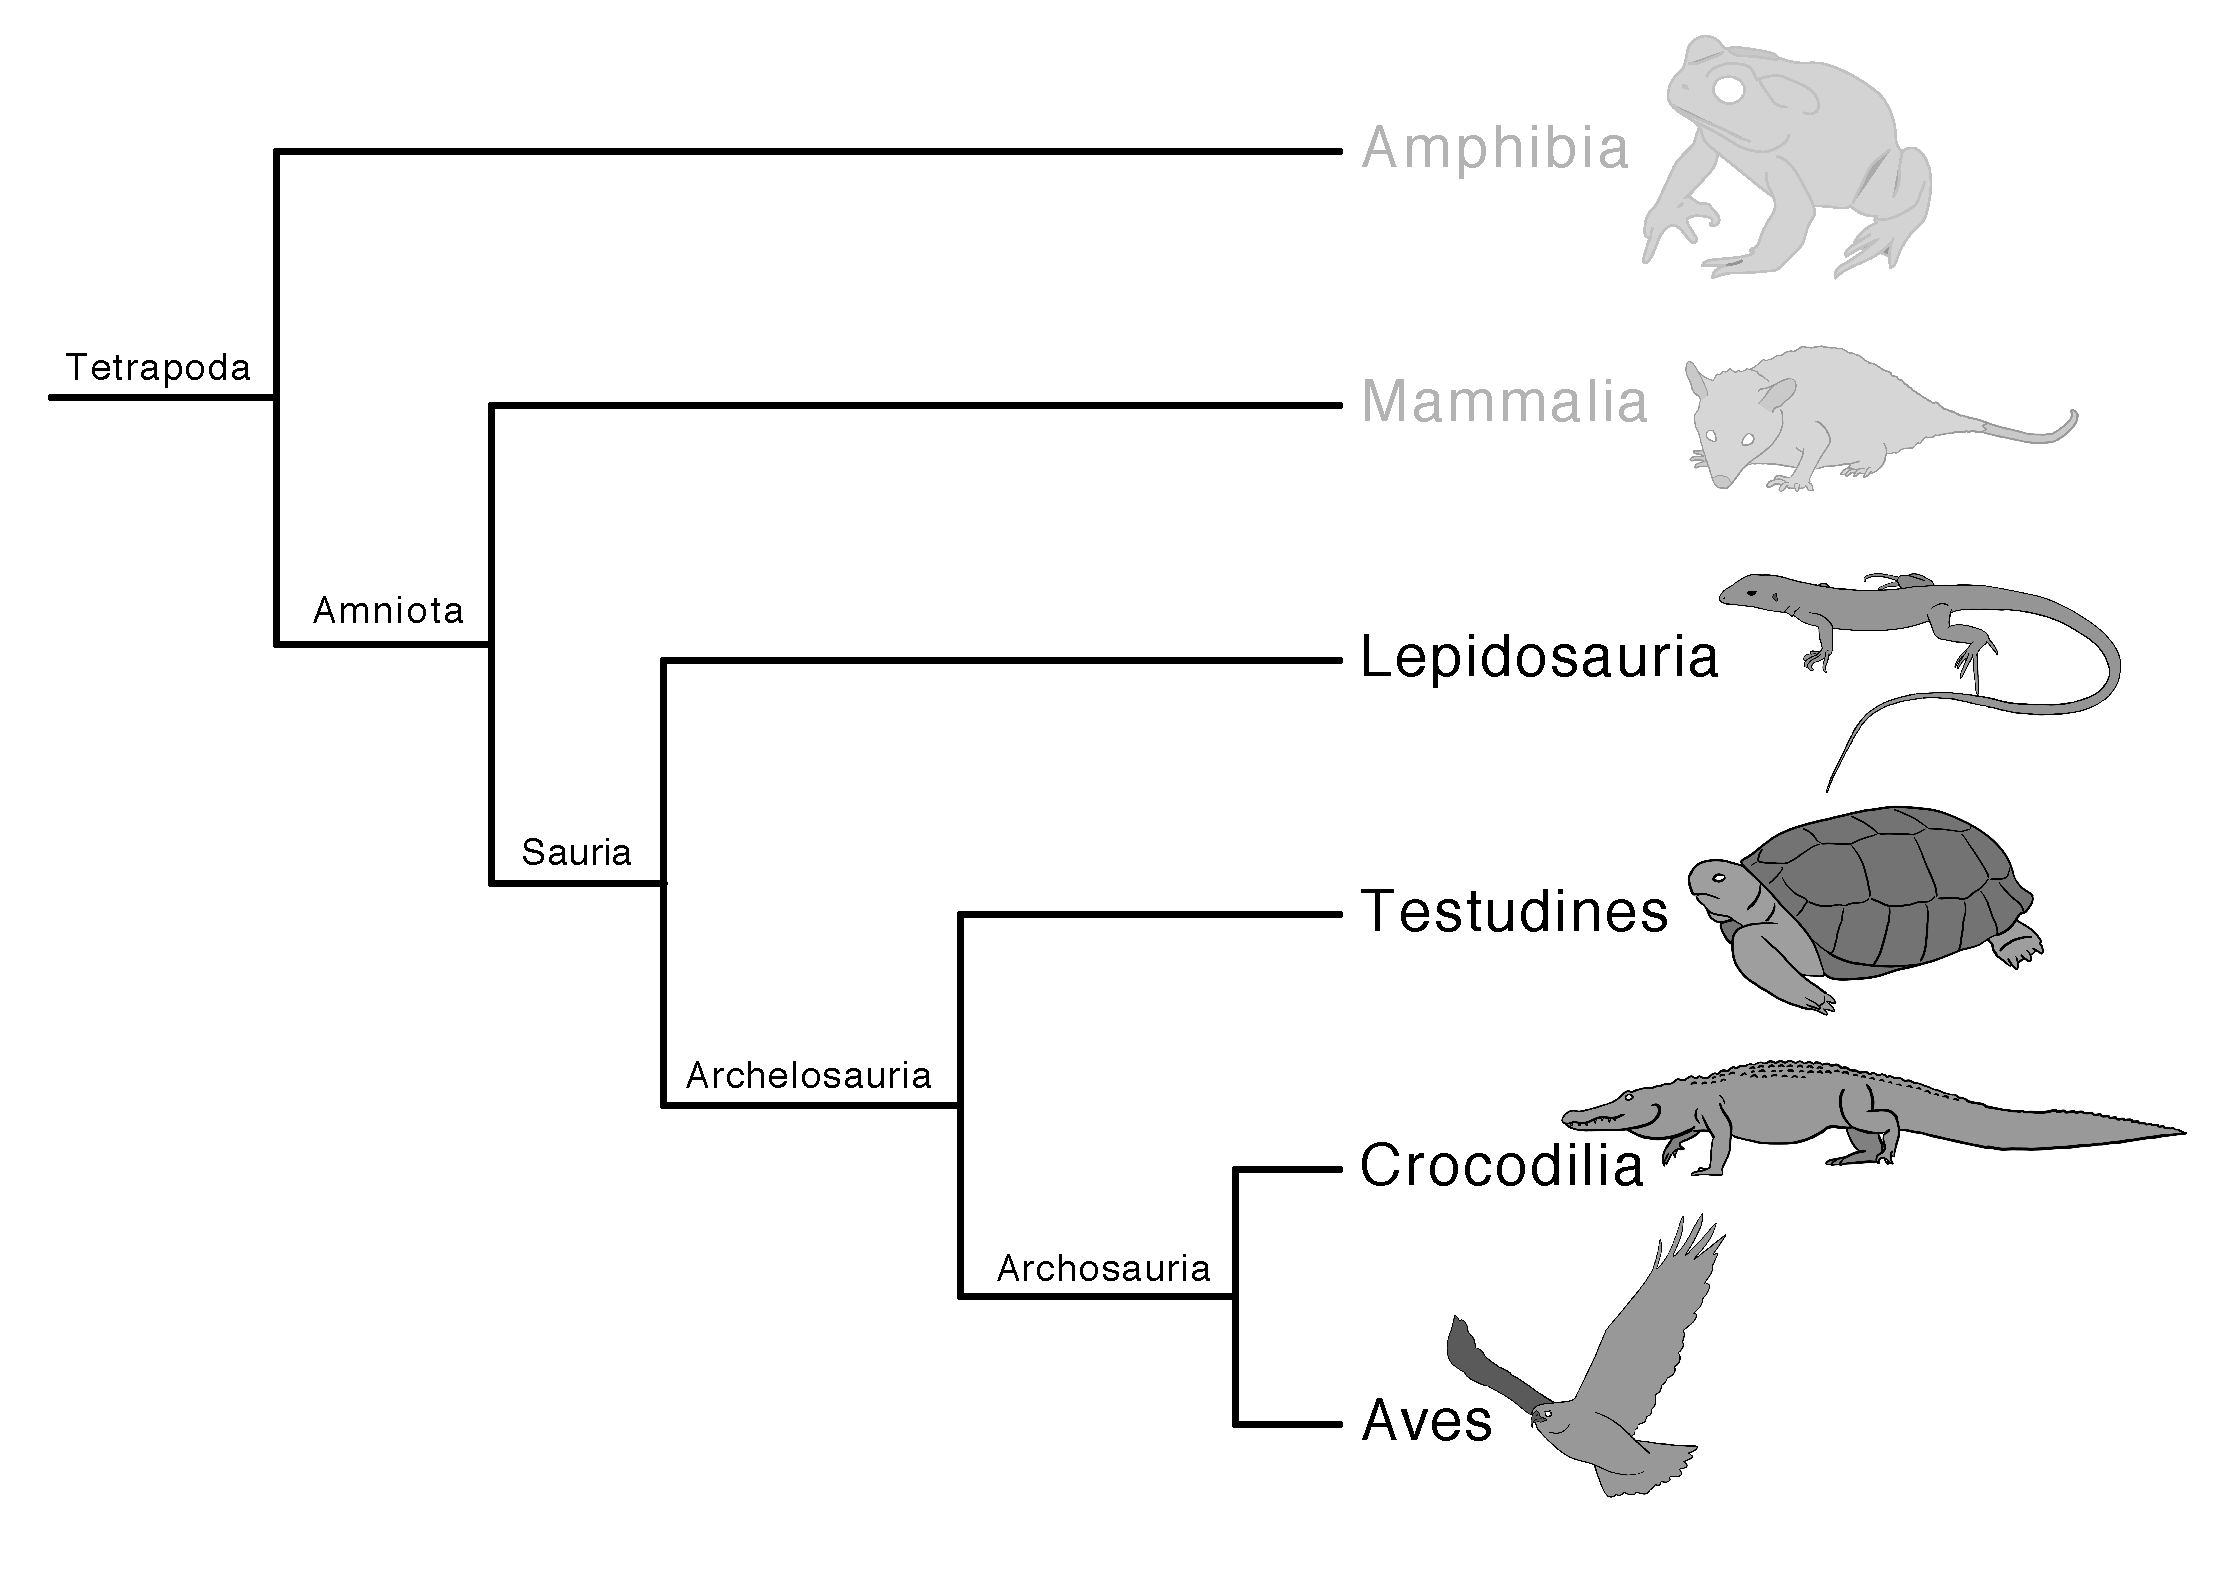
\includegraphics[scale=0.4]{Amniota_tre.pdf}
  \caption{Amniote Relationships}
  \label{fig:Amniota}
\end{figure}

\begin{figure}[H]
\centering
  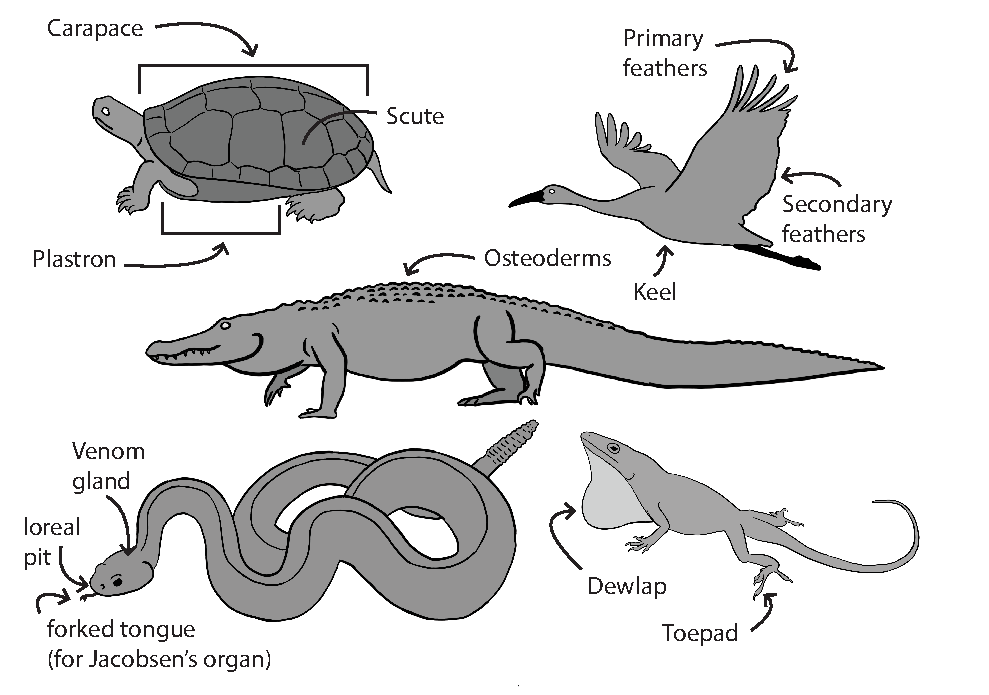
\includegraphics{DiapsidAnatomy.pdf}
  \caption{Diapsid anatomical terms to know}
  \label{fig:Anura}
\end{figure}

\section*{Focal taxonomic groups} ($\star$ groups you need to be able to photo ID and place in a phylogeny. $\mathsection$ denotes species for which you need to audio ID calls.)
\begin{description}

\begin{figure}[H]
\centering
  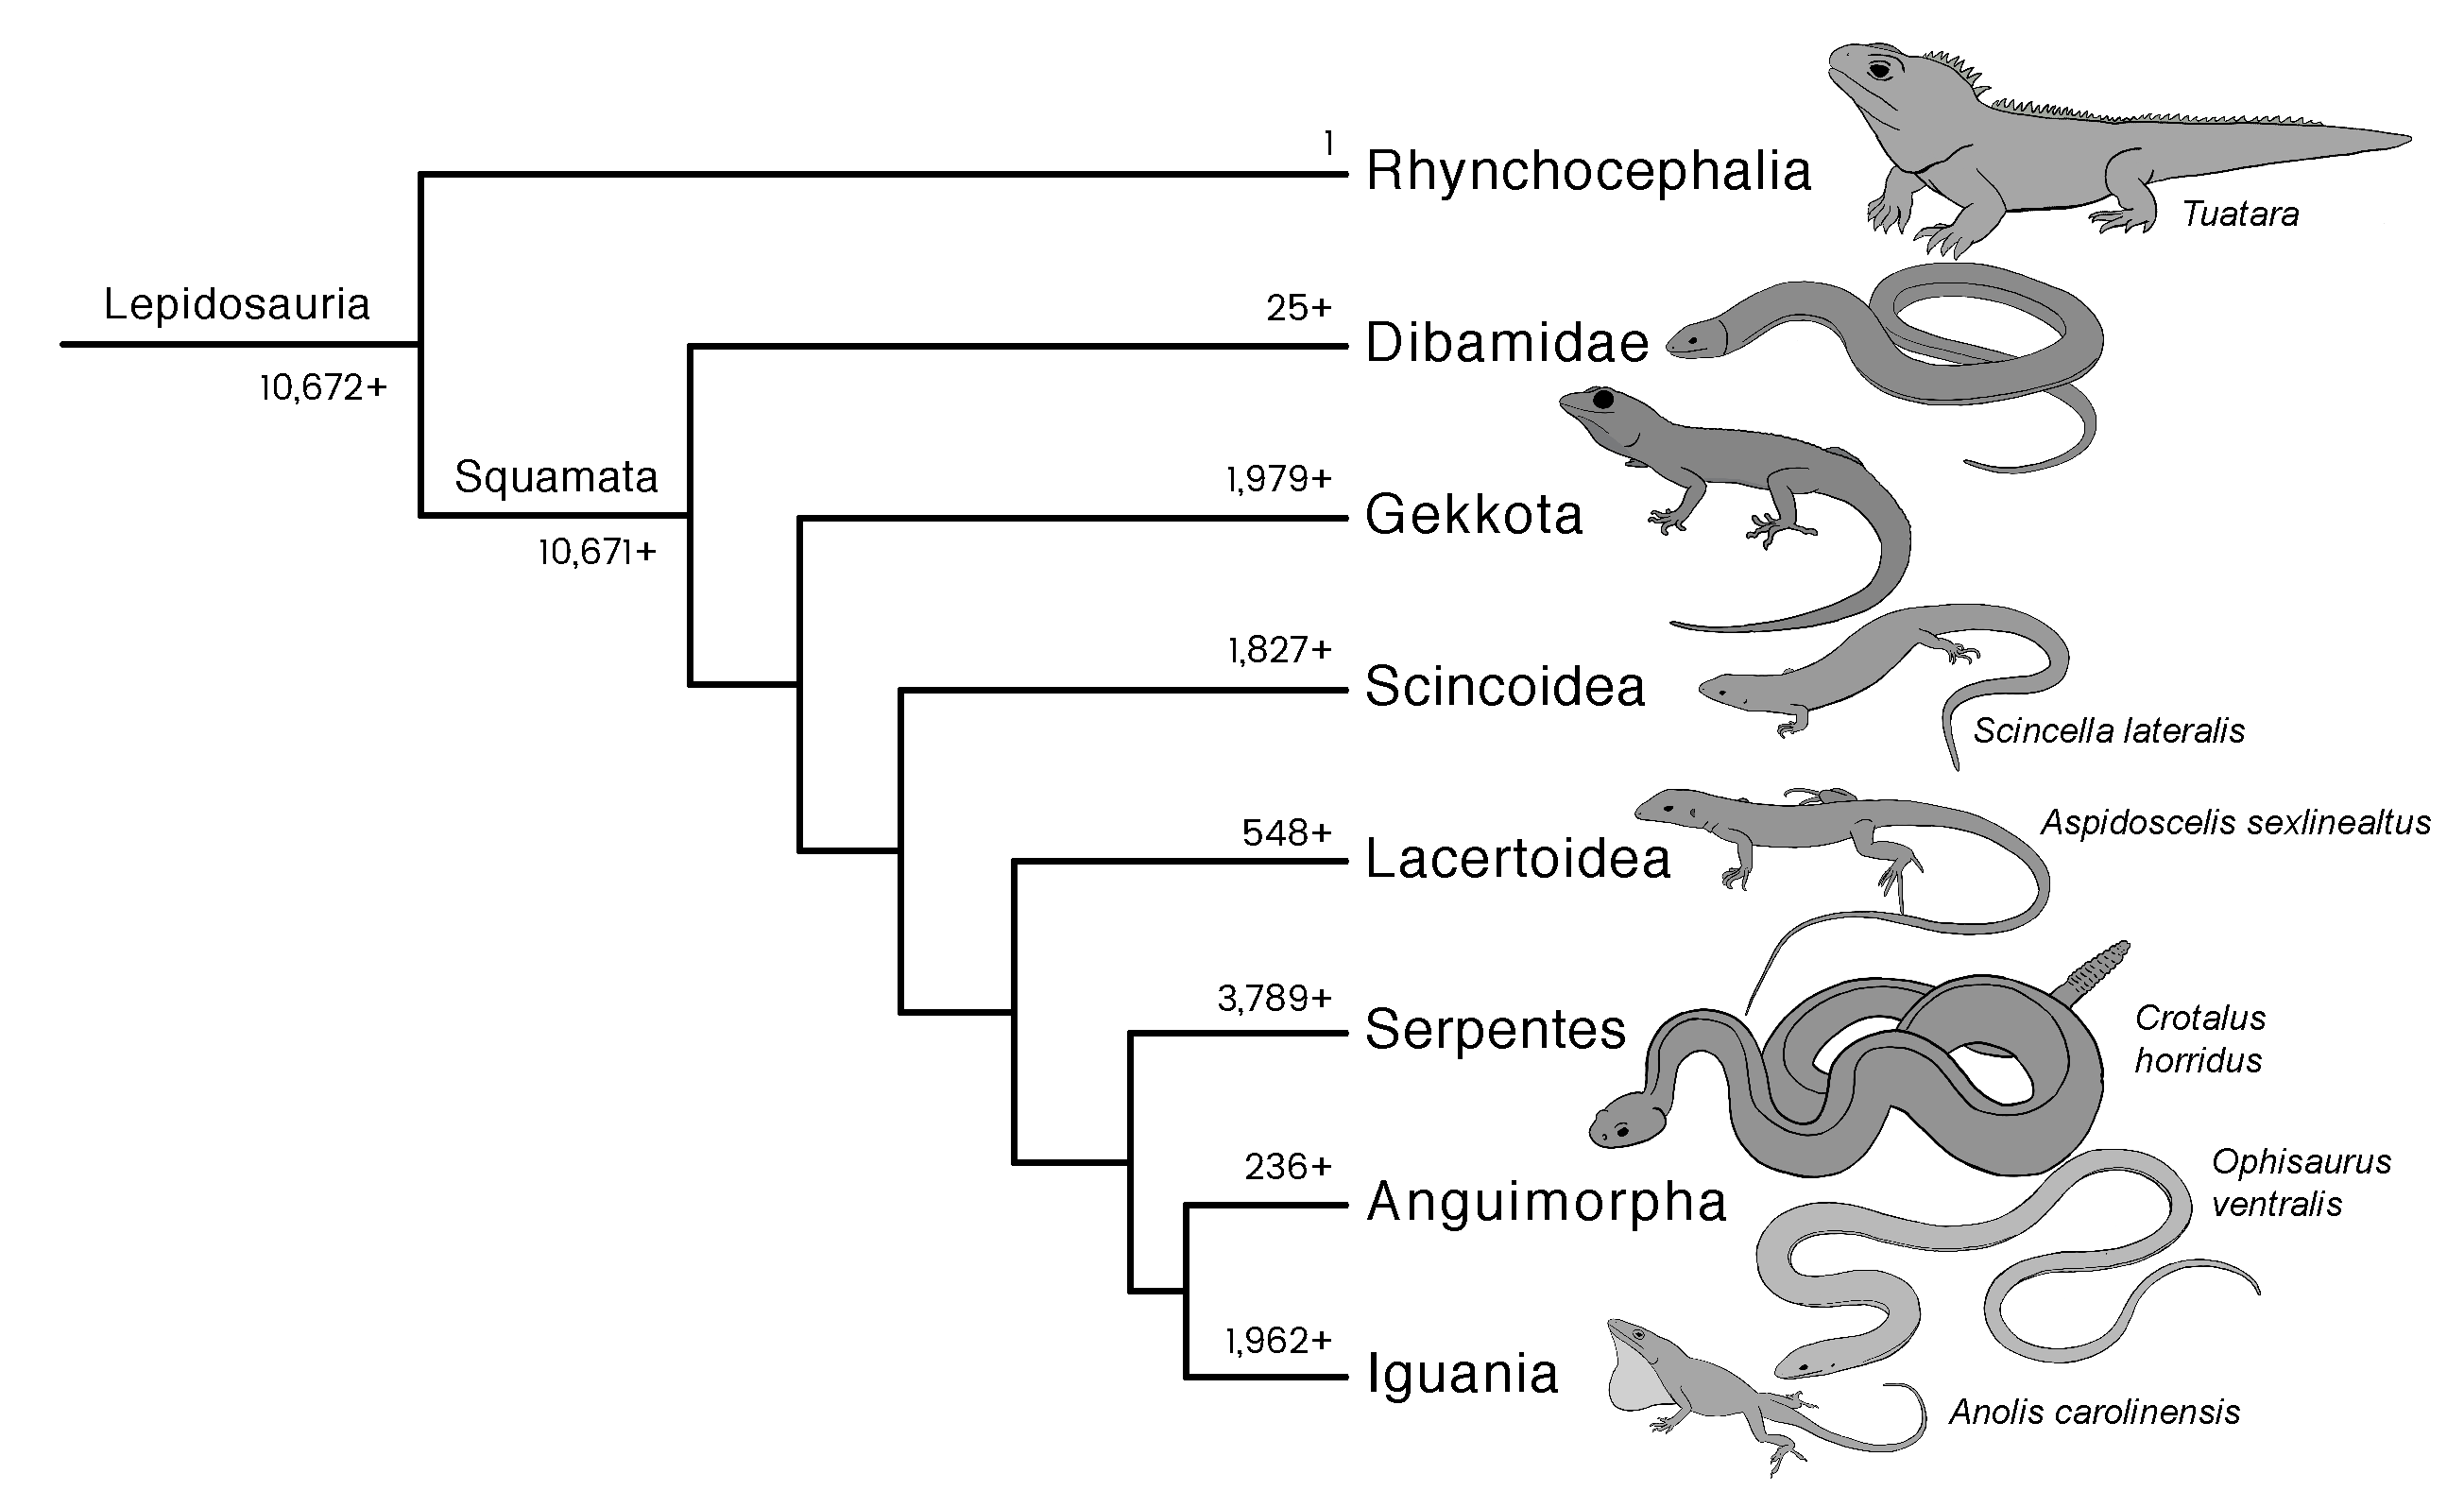
\includegraphics[scale=0.4]{Lepidosauria_tre.pdf}
  \caption{Lepidosaur Relationships}
  \label{fig:Lepidosauria}
\end{figure}

\item{\underline{{\LARGE{Lepidosauria}}}}
Transverse cloacal slit, regular cycles of shedding, tongue distally notched, paired copulatory organs, well-developed quadrate conch, ectepicondylar foramen in the humerus (median nerve and brachial artery passage), pleurodont dentition
\item\textbf{Rhynchocephalia} \\ Once distributed globally (most abundant group in South America during Cretaceous). No well defined hemipenes- paired copulatory organs are slight outpushings of cloacal walls. Gastralia present.
\begin{itemize}
  \item Family {\textbf{SPHENODONTIDAE} (tuatara$\star$)} \\ Only extant Rhynchocelphalian (one genus, two species). Ancestral diapsid skull (two temporal fenestra on either side of skull). One or both of these holes have been lost in lizards and snakes, respectively. Highly developed pineal gland (regulates circadian rhythm). Teeth fused to skull (sphenodont dentition), and become dull with time. A single row of teeth on the lower jaw fit between two rows on the upper jaw, a trait unique among all tetrapods. Tuatara can live upwards of 100 years. * No alcohol-preserved specimen, just skull replicate.
\end{itemize}
\item\textbf{Squamata} \\ Highly developed hemipenes (paired copulatory organs), Jacobsen's organ separated from nasal capsule, femoral and preanal glands, no gastralia, triradiate squamosal
\begin{itemize}
  \item Family {\textbf{DIBAMIDAE} (blind skinks)} \\ In these elongate lizards, males have tiny flap like hindlimbs and females are completelylimbless. They also lack external ear openings. All of these features are likely adaptations totheir fossorial lifestyle. They are found in Mexico and in Southeast Asia. Largely limbless (small flap-like hindlimbs in males). * No specimen.
  \item{\textbf{Gekkota} (geckos)$\star$}
  \begin{itemize}
    \item Family {\textbf{GEKKONIDAE} (spectacled geckos)} \\ Two species have been introduced to Alabama. They are readily identified by their lack eyelids and setae-covered toe pads. Toe pads with tiny hair like structures called setae. These toe pads enable them to climb vertical surfaces.
  \end{itemize}
  \item{\textbf{Scincoidea}}
  \begin{itemize}
    \item Family {\textbf{SCINCIDAE} (skinks)} \\ Dorsal scales smooth, shiny, and cicloid
    \begin{itemize}
      \item{\textbf{\textit{Scincella lateralis}} (ground skink)$\star$} \\ small skink, reduced limbs, bronzy color body with dark dorsolateral stripe. Transparent disc in lowereyelid.
      \item{\textbf{\textit{Plestiodon fasciatus}} (five-lined skink)$\star$} \\ Female has 5 broad light stripes down a black body; Male has traces of stripes,reddish jaws, juveniles have bright blue tails and 5 lines.
    \end{itemize}
  \end{itemize}
  \item{\textbf{Lacertoidea}} \\ Includes amphisbaenians, racerunners/whiptails, and tegus
  \begin{itemize}
    \item Family {\textbf{TEIIDAE}} \\ Have velvety textured dorsal scales and large, rectangular ventral scales, Pointed snout, Forked tougue, tail over 2x SVL, highly active foragers
    \begin{itemize}
      \item{\textbf{\textit{Aspidoscelis sexlineata$\star$}} (six-lined racerunner)} \\ six light lines on back, small dorsal scales. Large limb and ventral scales
    \end{itemize}
  \end{itemize}
    \item{\textbf{Anguimorpha}} \\ Group that contains the only venemous lizards (Helodermatidae and Varanidae) and Anguids.
  \begin{itemize}
    \item Family {\textbf{ANGUIDAE}} \\ Elongate lizards with reduced limbs or limbless. Scales usually rectangular. Lateral fold in most taxa.
    \begin{itemize}
      \item{\textbf{\textit{Ophisaurus ventralis}} (eastern glass lizard)$\star$} \\ No legs, has ear openings and moveable eyelids, smooth scales, dark dorsum light venter, generally gray-green.
    \end{itemize}
  \end{itemize}
  \item{\textbf{Iguania}} \\ Diverse group that includes acrodonts (Agamidae, Chamelonidae) and pleurodonts (Iguanidae, Corytophanidae, Crotaphytidae, Dactyloidae, and Phrynosomatidae)
  \begin{itemize}
    \item{\textbf{\textit{Anolis carolinensis}} (green anole)$\star$} \\ Have subdigital lamallae bearing setae much like gekkota. Males have prominent dewlaps. No pattern, relatively small individual scales, capable of changing between green and brown skin color, reddish dewlap, long slender body shape.
  \end{itemize}
  \item{\textbf{Serpentes} (snakes)}
  \begin{itemize}
    \item family {\textbf{VIPERIDAE}} (vipers) \\ Crotalinae (restricted to Eurasia \& Americas) have heat-sensing pit between eye and nostril; paired single tooth on maxilla (mobile fang) that functions to deliver potent venom (many species possess neurotoxic, hemotoxic, and cytotoxic venom- some with a cocktail), broad head, vertical pupil. Many species are viviparous.
    \begin{itemize}
      \item{\textbf{\textit{Crotalus horridus}} (timber rattlesnake)$\star$} \\ variable but always with dark chevron-like cross bands on light background that gets darker towards tail, reddish brown middorsal stripe, dark postocular line
    \end{itemize}
    \item family {\textbf{ELAPIDAE}} (elapids) \\ Venomous snakes endemic to tropical and subtropical regions. Some snakes are aquatic (e.g., kraits). Longest venemous snake (king cobra). Fixed fangs at front of upper jaw for injecting venom, which is largely made up of neurotoxic compounds.
    \begin{itemize}
      \item{\textbf{\textit{Micrurus fulvius}} (eastern coralsnake)$\star$} \\ Have smooth scales, black snout, and aposomatic red and yellow banding pattern. They have a hand full of mimics which in the U.S. can be differentiated by the order of colored bands. A useful rhyme is "Red touching black, friend of Jack. Red touching yellow, kill a fellow."
    \end{itemize}
    \item family {\textbf{COLUBRIDAE}} \\ Lack heat-sensing pits; have multiple teeth onmaxilla. Make up 78\% of world’s snakespecies.
    \begin{itemize}
      \item{\textbf{\textit{Pantherophis spiloides}} (gray rat snake)$\star$} \\ ``loaf of bread'' body shape, variable but light grayish body with darker blotches downback, divided anal plate.
      \item{\textbf{\textit{Nerodia sipedon}} (midland brown water snake)$\star$} \\ keeled scales, belly has double row of crescents, back has dark markings that are narrower than the light spaces between them.
    \end{itemize}
  \end{itemize}
\end{itemize}

\begin{figure}[H]
\centering
  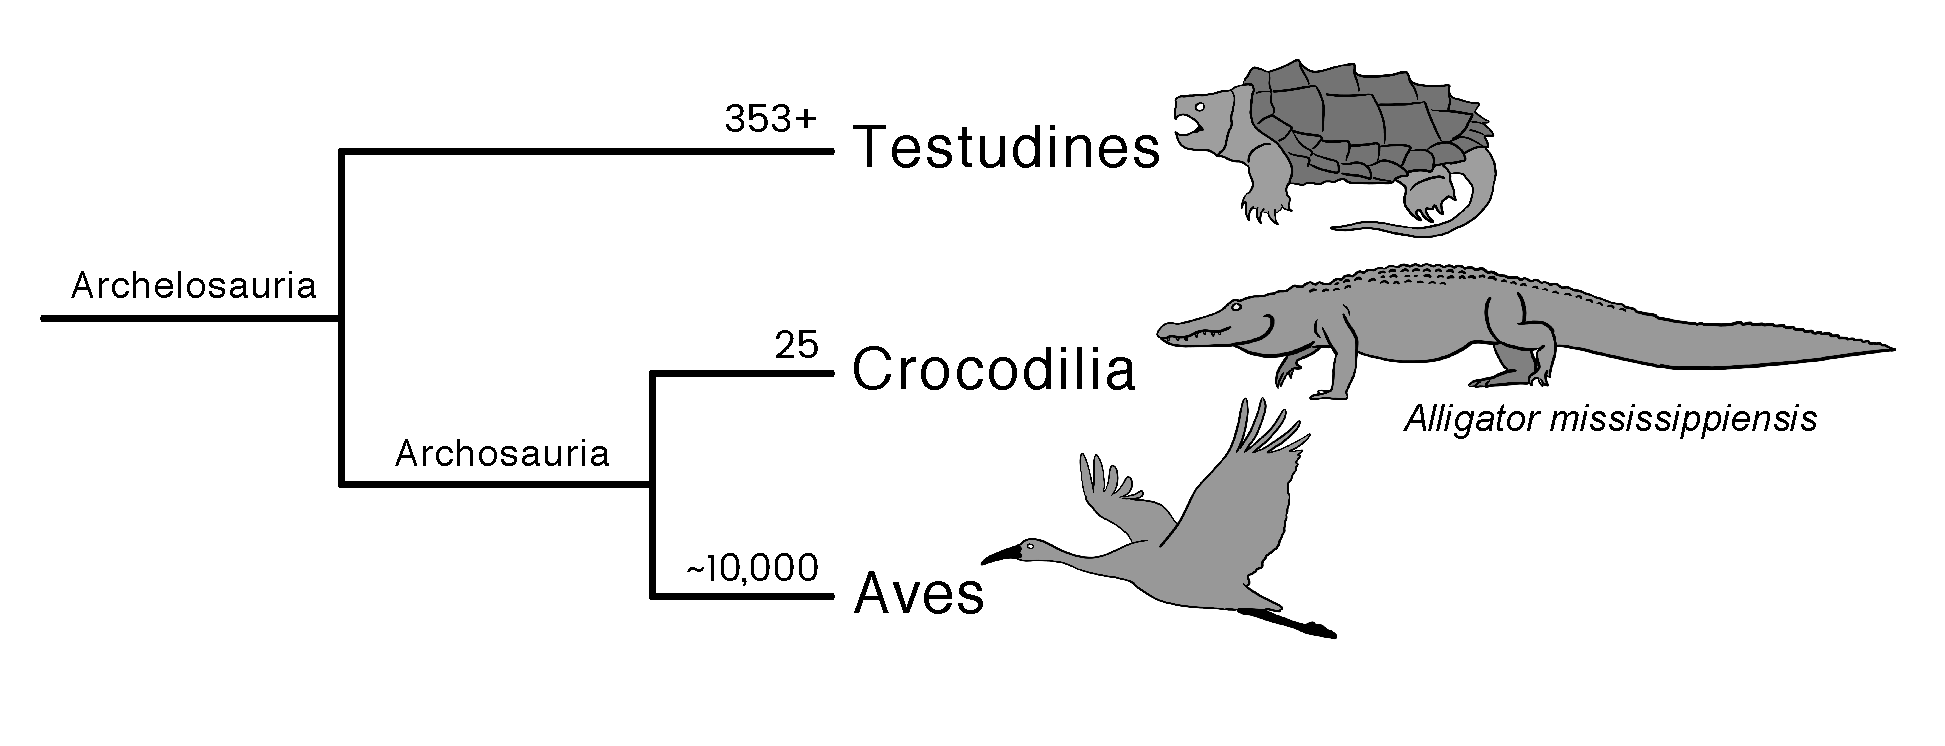
\includegraphics[scale=0.3]{Archelosauria_tre.pdf}
  \caption{Archelosaur Relationships}
  \label{fig:Archelosauria}
\end{figure}


\item{\underline{{\LARGE{Archelosauria}}}}
While phylogenetic conclusions from morphological analyses conflict with those from genetic analyses, most systematists place testudines as sister to the group encompassing crocodylians and aves (Archosauria). This larger group (Archelosauria) lacks diagnostic anotomical characters, but thorough molecular data consistently recover the three groups together.

\item\textbf{Crocodilia} \\ Robust skull, long snout, strongly toothed jaws, short neck, robust cylindrical trunk, laterally compressed tail, short but strongly developed limbs with webbed feet. Largest living reptiles. Bony plates (osteoderms) covered by keratinou skin provide armor to neck, trunk, and tail. All crocodylians are oviparous with internal fertilization, and have temperature-dependent sex determination. 

\begin{itemize}
  \item{\textbf{\textit{Alligator mississippiensis}} (American alligator)$\star$} \\ Broad snout, large body, fourth mandibular tooth hidden when mouth is closed.
\end{itemize}

\begin{figure}[H]
\centering
  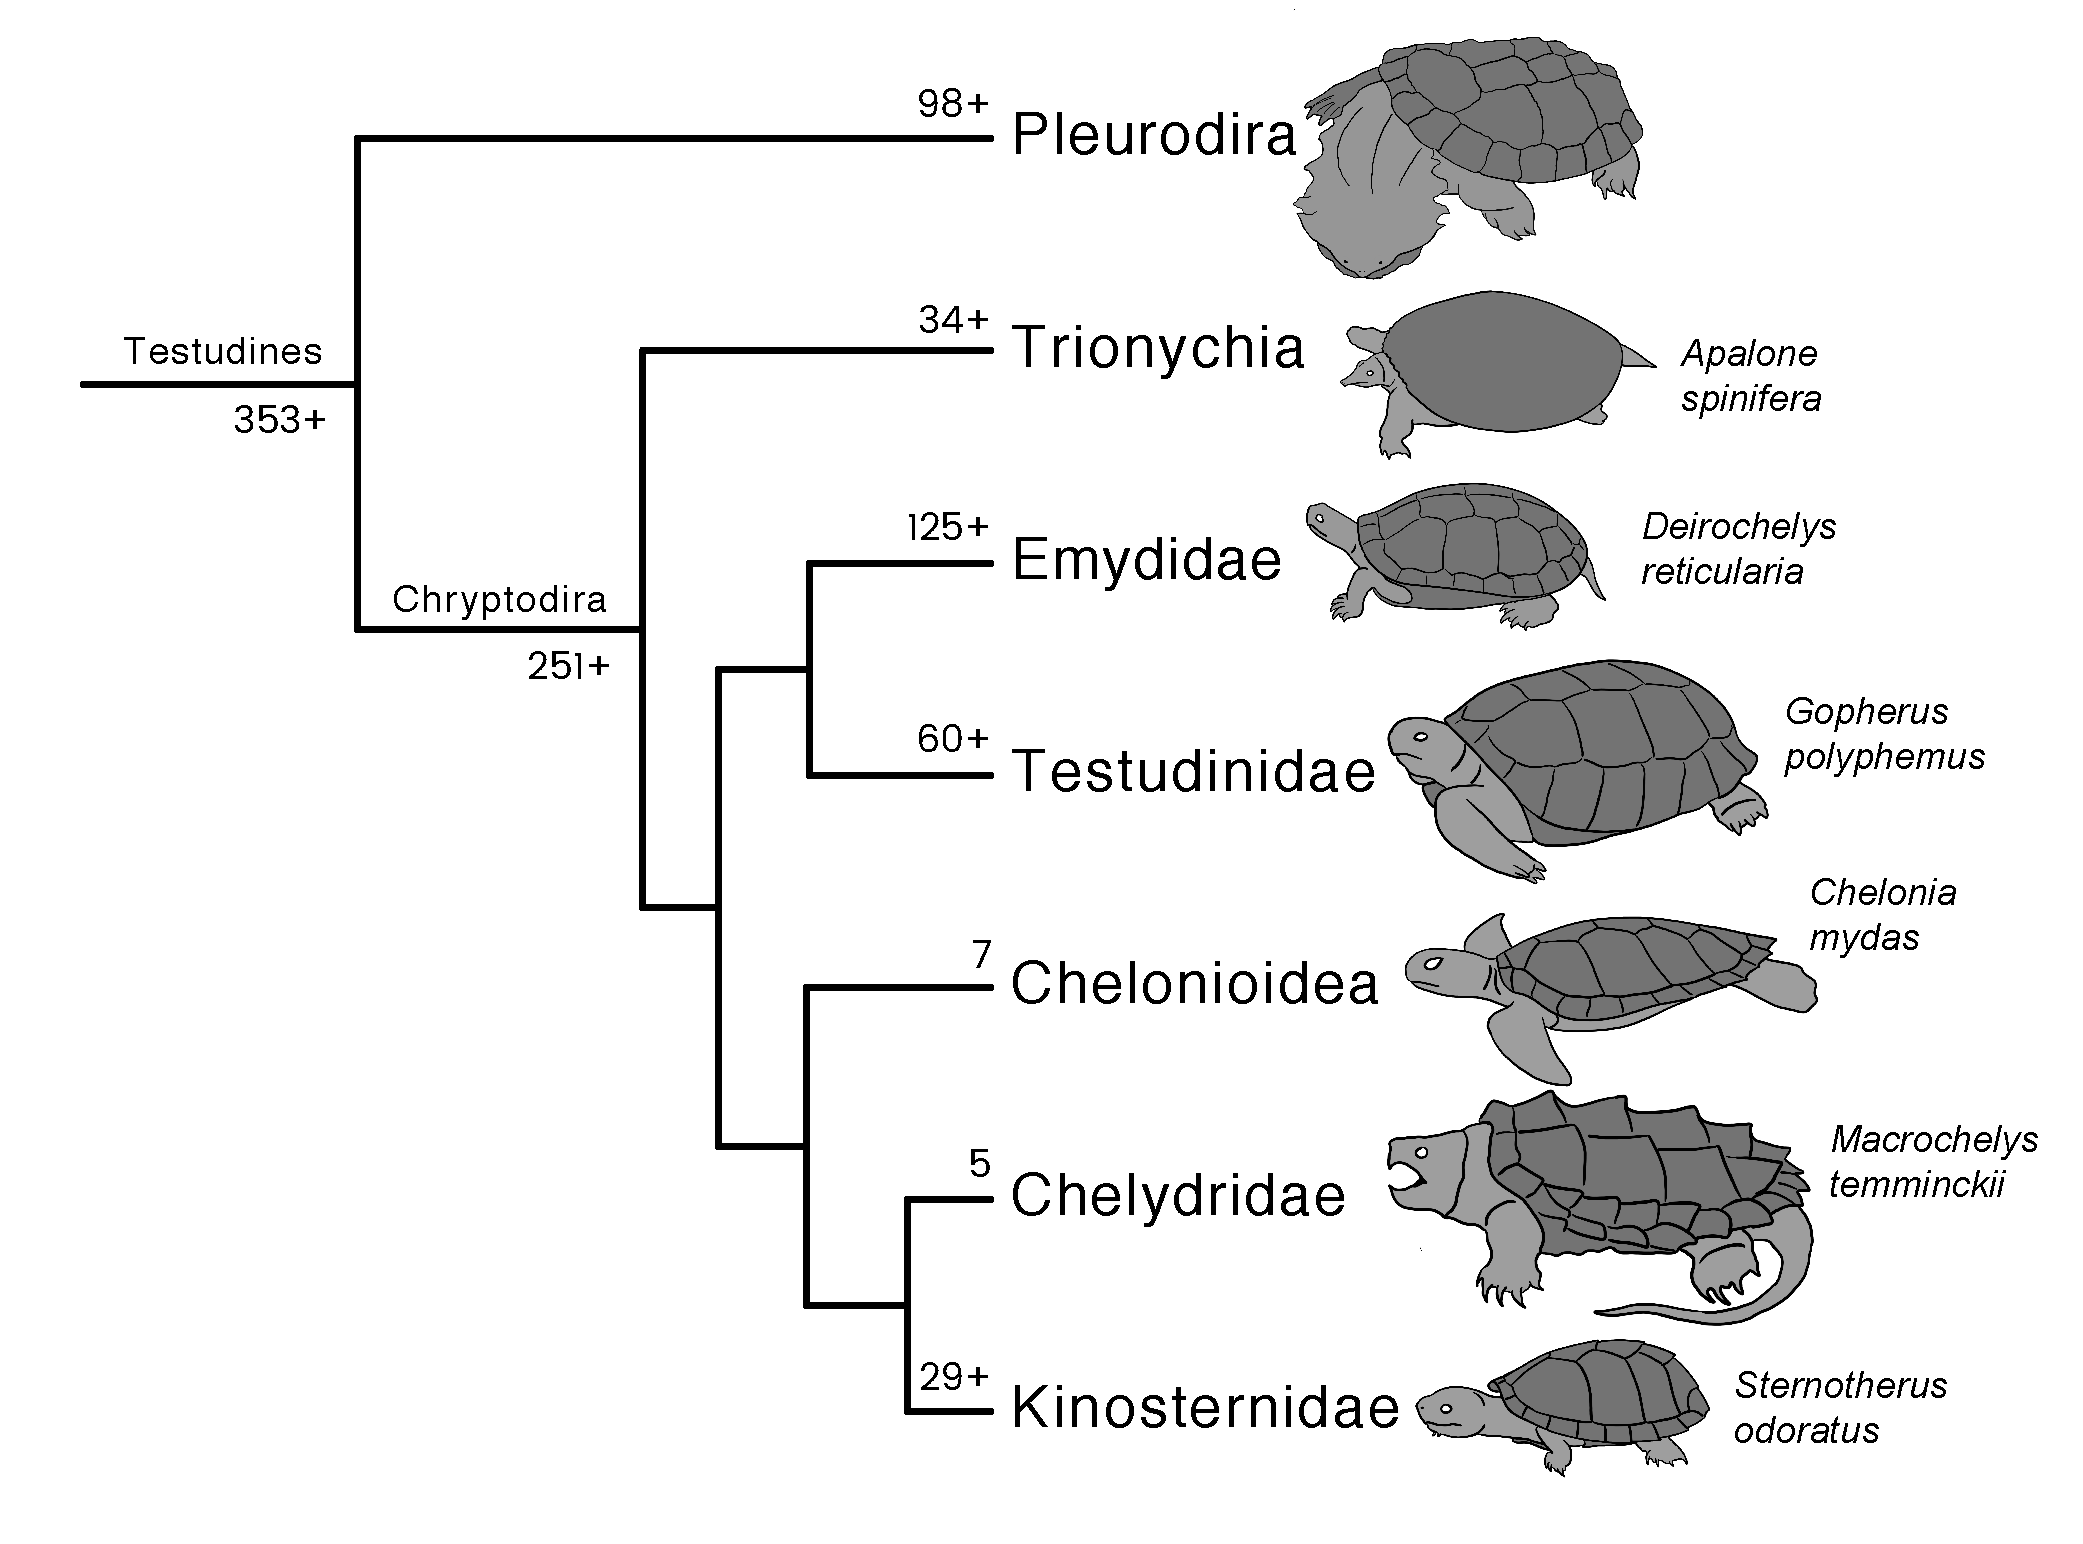
\includegraphics[scale=0.4]{Testudines_tre.pdf}
  \caption{Testudine Relationships}
  \label{fig:Testudines}
\end{figure}


\item\textbf{Testudines} \\ Reptilian tanks- no other tetrapod with bony shell that encloses the pectoral and pelvic girdles. The carapace (dorsal portion of the shell) is made up of 8 trunk vertebrae fused with ribs and overlying dermal bones. The plastron (ventral portion of the shell) is made up of the sternum and gastralia fused with external dermal bones. The neck is made up of 8 cervical vertebrae. All turtles are oviparous with internal fertilization, and many have temperature-dependent sex determination.

\begin{itemize}
  \item{\textbf{Pleurodira} (side-neck turtles)} \\ Withdraw head and neck laterally within the outer margin of the shell
  \item{\textbf{Cryptodira} (S-neck turtles)} \\ Withdraw head and neck within shell in S-shape
  \begin{itemize}
    \item {\textbf{Trionychia} (softshell turtles)} \\ Flat, pancake shells, no epidermal scutes
    \begin{itemize}
      \item{\textbf{\textit{Apalone spinifera}} (spiny softshell)$\star$} \\ Anterior carapacial tubercles often pointed or spine-tipped. Hatchlings with spotted carapace that becomes uniformally dark with age
    \end{itemize}
    \item Family {\textbf{EMYDIDAE} (pond turtles)} \\ Moderately domed carapace, tear-drop shaped carapace
    \begin{itemize}
      \item{\textbf{\textit{Deirochelys reticularia}} (chicken turtle)$\star$} \\ Pair of dark spots on bridge, sholder-to-snout length as long as plastron
    \end{itemize}
    \item Family {\textbf{TESTUDINIDAE} (tortoises)} \\ Terrestrial; forelimbs shovel-like for digging, hind feet elephantine for walking.
    \begin{itemize}
      \item{\textbf{\textit{Gopherus polyphemus} (gopher tortoise)$\star$}} \\ Carapace is oblong, flat-topped, and drops off abruptly on the sides and at the rear.
    \end{itemize}
    \item {\textbf{CHELONIOIDEA} (sea turtles)} \\ Limbs modified into flippers, streamlined shell
    \begin{itemize}
      \item{\textbf{\textit{Chelonia mydas} (green sea turtle)$\star$}} \\ Scutes of carapace not overlapping, 4 pleural scutes
    \end{itemize}
    \item {\textbf{CHELYDRIDAE} (snapping turtles)} \\ Large head, flattened carapace, long tails (about as long as carapace)
    \begin{itemize}
      \item{\textbf{\textit{Chelydra serpentina} (alligator snapping turtle)$\star$}} \\ Long tail, hooked beak, Three large longitudinal ridges on carapace. Largest turtle in North America
    \end{itemize}
    \item {\textbf{KINOSTERNIDAE} (mud and musk turtles)} \\ Plastron with 10 or 11 scutes, defined overhanging beak, potato-like (oblong) shape
    \begin{itemize}
      \item{\textbf{\textit{Sternotherus odoratus} (common musk turtle)$\star$}} \\ paired barbels on both chin and neck. 
    \end{itemize}
  \end{itemize}
\end{itemize}


\begin{figure}[H]
\centering
  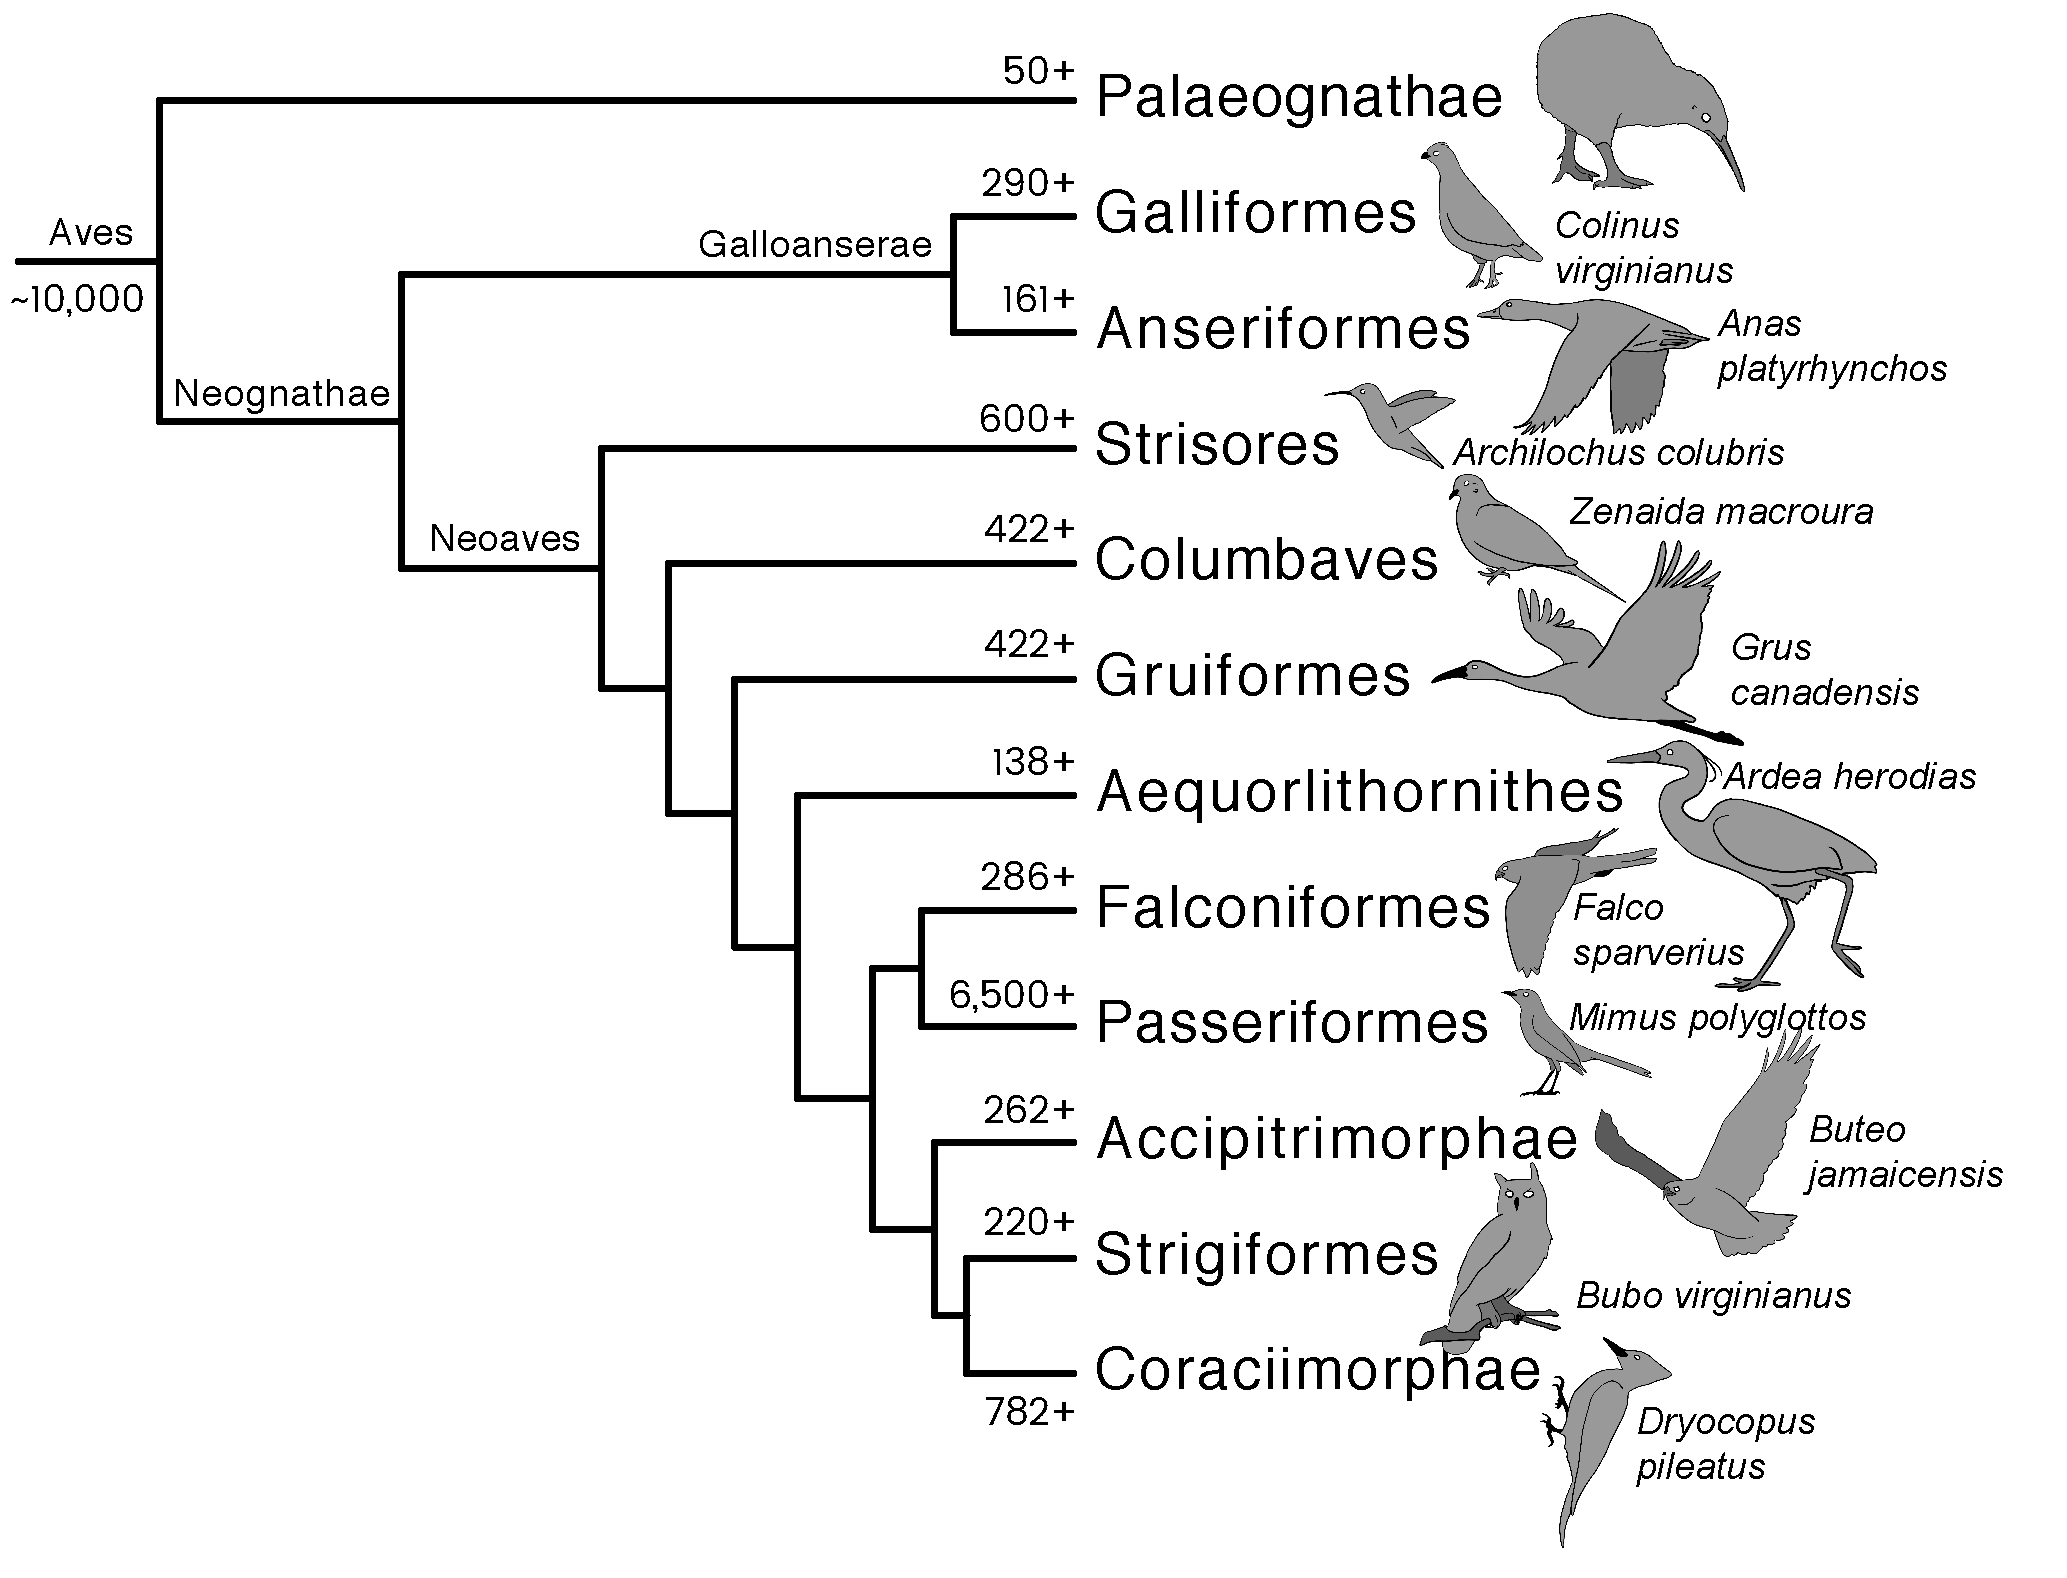
\includegraphics[scale=0.3]{Aves_tre.pdf}
  \caption{Ave Relationships}
  \label{fig:Aves}
\end{figure}

\item\textbf{Aves} \\ Front limbs modified into wings, scales modified into feathers (for thermoregulation and flight), bone structure and density reduced to reduce weight for flight.

\begin{itemize}
  \item Family {\textbf{PALAEOGNATHAE}} \\ Flightless birds with rigid palate. Largest bird (ostrich) and the small kiwi both belong to this group.
  \item Family {\textbf{NEOGNATHAE}} \\ Fused metacarpals, elongate third finger
  \begin{itemize}
    \item {\textbf{Galliformes}} \\ Heavy-bodied, ground-feeding birds (including turkey, grouse, chicken, quail, pheasent). This lineage survived the K-T mass extinction. It is hypothesized that their small ground-dwelling nature allowed them to outlive their abundant airborne relatives.
    \begin{itemize}
      \item{\textbf{\textit{Colinus virginianus}} (northern bobwhite)$\star$ $\mathsection$} \\ small quail with rounded bodies, small head, rounded tail, and short wings. Males have a bold black-and-white head pattern. Females have a buffy throat and eyebrow.
    \end{itemize}
    \item {\textbf{Anseriformes}} \\ Water-adapted birds (including ducks, geese, and swans), which niche is hypothesized to have helped them survive the K-T mass extinction.
    \begin{itemize}
      \item{\textbf{\textit{Anas platyrhynchos}} (mallard)$\star$ $\mathsection$} \\ Heavy-bodied dabbling duck native to North America, Eurasia, and North Africa. Breeding males have glossy bottle-green heads and a demarcating white collar, pale gray belly, purple-tinged brown breast, and a bill that is yellow-orange and tipped with black. Female is predominantly mottled. Both males and females have iridescent blue-purple speculum (wing) feathers.
    \end{itemize}
    \item {\textbf{Strisores}} \\ Torpor (hibernation-like state) along with other unique metabolic traits are common in this group of birds (including nightjars, swifts, hummingbirds, potoos, frogmouths)
    \begin{itemize}
      \item{\textbf{\textit{Archilochus colubris}} (Ruby-throated hummingbird)$\star$} \\ The Ruby-throated Hummingbird is a small hummingbird with a slender, slightly downcurved bill and fairly short wings that don’t reach all the way to the tail when the bird is sitting. Ruby-throated Hummingbirds are bright emerald or golden-green on the back and crown, with gray-white underparts. Males have a brilliant iridescent red throat that looks dark when it’s not in good light.
    \end{itemize}
    \item {\textbf{Columbaves}} \\ Relatively new description of a group that includes pigeons, doves, mesites, and cuckoos, turacos, and bustards
    \begin{itemize}
      \item{\textbf{\textit{Zenaida macroura}} (Mourning dove)$\star$ $\mathsection$} \\ Plump-bodied and long-tailed, with short legs, small bill, and a head that looks particularly small in comparison to the body. The long, pointed tail is unique among North American doves. Mourning Doves often match their open-country surroundings. They’re delicate brown to buffy-tan overall, with black spots on the wings and black-bordered white tips to the tail feathers.
    \end{itemize}
    \item {\textbf{Gruiformes}} \\ Group of wading birds (including cranes, crakes, rails). Globally distributed.
    \begin{itemize}
      \item{\textbf{\textit{Fulica americana}} (American coot)$\star$} \\ The American Coot is a plump, chickenlike bird with a rounded head and a sloping bill. Their tiny tail, short wings, and large feet are visible on the rare occasions they take flight. Coots are dark-gray to black birds with a bright-white bill and forehead. The legs are yellow-green. At close range you may see a small patch of red on the forehead.
      \item{\textbf{\textit{Grus canadensis}} (Sandhill Crane)$\star$} \\ Sandhill Cranes are very large, tall birds with a long neck, long legs, and very broad wings. These are slate gray birds, often with a rusty wash on the upperparts. Adults have a pale cheek and red skin on the crown.
    \end{itemize}  
    \item {\textbf{Aequorlitornithes}} \\ Water and shore birds (including flamingos, grebes, shorebirds, loons, penguins, herons, pelicans, gulls). Globally distributed. These birds were grouped relatively recently.
    \begin{itemize}
      \item{\textbf{\textit{Ardea herodias}} (Great Blue Heron)$\star$} \\ Largest of the North American herons with long legs, a sinuous neck, and thick, daggerlike bill. Head, chest, and wing plumes give a shaggy appearance. In flight, the Great Blue Heron curls its neck into a tight “S” shape; its wings are broad and rounded and its legs trail well beyond the tail. Great Blue Herons appear blue-gray from a distance, with a wide black stripe over the eye. In flight, the upper side of the wing is two-toned: pale on the forewing and darker on the flight feathers. A pure white subspecies occurs in coastal southern Florida.
      \item{\textbf{\textit{Leucophaeus atricilla}} (Laughing Gull)$\star$ $\mathsection$} \\ Laughing Gulls are medium-sized gulls with fairly long wings and long legs that impart a graceful look when they are flying or walking. They have stout, fairly long bills. Laughing Gulls are medium gray above and white below. Summer adults have a crisp black hood, white arcs around the eye, and a reddish bill. In winter, the hood becomes a blurry gray mask on a white head. The legs are reddish black to black. Immatures are much browner and more subtly patterned than adults; they take 2-3 years to gain adult plumage.
    \end{itemize} 
    \item {\textbf{Accipitrimorphae}} \\ Large birds of prey (including New World vultures, eagles, hawks, eagles, osprey, and secretarybird).
    \begin{itemize}
      \item{\textbf{\textit{Cathartes aura}} (Turkey Vulture)$\star$} \\ Turkey Vultures are large dark birds with long, broad wings. Bigger than other raptors except eagles and condors, they have long "fingers" at their wingtips and long tails that extend past their toe tips in flight. When soaring, Turkey Vultures hold their wings slightly raised, making a ‘V’ when seen head-on. Turkey Vultures appear black from a distance but up close are dark brown with a featherless red head and pale bill. While most of their body and forewing are dark, the undersides of the flight feathers (along the trailing edge and wingtips) are paler, giving a two-toned appearance.
      \item{\textbf{\textit{Buteo jamaicensis}} (Red-tailed Hawk)$\star$ $\mathsection$} \\ Red-tailed Hawks are large hawks with typical Buteo proportions: very broad, rounded wings and a short, wide tail. Most Red-tailed Hawks are rich brown above and pale below, with a streaked belly and, on the wing underside, a dark bar between shoulder and wrist. The tail is usually pale below and cinnamon-red above, though in young birds it’s brown and banded. “Dark-morph” birds are all chocolate-brown with a warm red tail. “Rufous-morph” birds are reddish-brown on the chest with a dark belly.
    \end{itemize}
    \item {\textbf{Strigiformes} (owls)} \\ Mostly solitary and nocturnal birds of prey typified by an upright stance, a large, broad head, binocular vision, binaural hearing, sharp talons, and feathers adapted for silent flight. Feed primarily on small mammals, insects, and other birds. Global distribution (with exception of polar ice caps and some remote islands).
    \begin{itemize}
      \item{\textbf{\textit{Bubo virginianus}} (Great Horned Owl)$\star$ $\mathsection$} \\ These are large, thick-bodied owls with two prominent feathered tufts on the head. The wings are broad and rounded. Great Horned Owls are mottled gray-brown, with reddish brown faces and a neat white patch on the throat.
    \end{itemize}
    \item {\textbf{Coraciimorphae} (woodpeckers and kingfishers)}
    \begin{itemize}
      \item{\textbf{\textit{Megaceryle alcyon}} (Belted Kingfisher)$\star$} \\ Belted Kingfishers are stocky, large-headed birds with a shaggy crest on the top and back of the head and a straight, thick, pointed bill. Their legs are short and their tails are medium length and square-tipped. These kingfishers are blue-gray above with fine, white spotting on the wings and tail. The underparts are white with a broad, blue breast band. Females also have a broad rusty band on their bellies. Juveniles show irregular rusty spotting in the breast band.
      \item{\textbf{\textit{Dryocopus pileatus}} (Pileated Woodpecker)$\star$ $\mathsection$} \\ The Pileated Woodpecker is a very large woodpecker with a long neck and a triangular crest that sweeps off the back of the head. The bill is long and chisel-like, about the length of the head. In flight, the wings are broad and the bird can seem crowlike. Pileated Woodpeckers are mostly black with white stripes on the face and neck and a flaming-red crest. Males have a red stripe on the cheek. In flight, the bird reveals extensive white underwings and small white crescents on the upper side, at the bases of the primaries.
    \end{itemize}
    \item {\textbf{Falconiformes} (falcons and caracaras)} \\ Small to medium-sized diurnal birds of prey with cosmopolitan distribution
    \begin{itemize}
      \item{\textbf{\textit{Falco sparverius}} (American Kestrel)$\star$} \\ The slender American Kestrel is roughly the size and shape of a Mourning Dove, although it has a larger head; longer, narrow wings; and long, square-tipped tail. In flight, the wings are often bent and the wingtips swept back. American Kestrels are pale when seen from below and warm, rusty brown spotted with black above, with a black band near the tip of the tail. Males have slate-blue wings; females’ wings are reddish brown. Both sexes have pairs of black vertical slashes on the sides of their pale faces—sometimes called a “mustache” and a “sideburn."
    \end{itemize}
    \item {\textbf{Passeriformes} (perching birds)} \\ More than half of all bird species. Three toes point forward and one points back.
    \begin{itemize}
      \item{\textbf{\textit{Corvus brachyrhynchos}} (American Crow)$\star$ $\mathsection$} \\ A large, long-legged, thick-necked bird with a heavy, straight bill. In flight, the wings are fairly broad and rounded with the wingtip feathers spread like fingers. The short tail is rounded or squared off at the end. American Crows are all black, even the legs and bill. When crows molt, the old feathers can appear brownish or scaly compared to the glossy new feathers.
      \item{\textbf{\textit{Mimus polyglottos}} (Northern Mockingbird)$\star$ $\mathsection$} \\ A medium-sized songbird, a bit more slender than a thrush and with a longer tail. Mockingbirds have small heads, a long, thin bill with a hint of a downward curve, and long legs. Their wings are short, rounded, and broad, making the tail seem particularly long in flight. Mockingbirds are overall gray-brown, paler on the breast and belly, with two white wingbars on each wing. A white patch in each wing is often visible on perched birds, and in flight these become large white flashes. The white outer tail feathers are also flashy in flight.
      \item{\textbf{\textit{Cardinalis cardinalis}} (Northern Cardinal)$\star$ $\mathsection$} \\ The Northern Cardinal is a fairly large, long-tailed songbird with a short, very thick bill and a prominent crest. Cardinals often sit with a hunched-over posture and with the tail pointed straight down. Male cardinals are brilliant red all over, with a reddish bill and black face immediately around the bill. Females are pale brown overall with warm reddish tinges in the wings, tail, and crest. They have the same black face and red-orange bill.
    \end{itemize}
  \end{itemize}
\end{itemize}
\end{description}

\end{document}
